\documentclass{article}
\usepackage{graphicx}
\usepackage{bm}
\usepackage{datetime2}
\usepackage{amsmath}
\usepackage{amssymb}
%\usepackage{unicode-math}
\usepackage{amsfonts} 
\usepackage{afterpage}
\usepackage{indentfirst}
\usepackage[margin=1in]{geometry} 
\usepackage{nameref}
\usepackage{booktabs}
\usepackage{latexsym}
\numberwithin{equation}{section}
\numberwithin{figure}{section}
\usepackage{caption}
\usepackage{float}
\usepackage{color}


\title{ Steady State Lid Driven Cavity Using Simple Algorithm - Finite Volume Method}
\author{Ganesh Borde}
\date{December 2024}
\begin{document}
\maketitle
\begin{abstract}
    This project focuses on the numerical simulation of flow inside a two-dimensional lid-driven 
    cavity. The study investigates the flow properties at low Reynolds numbers to 
    achieve a steady-state solution. A pressure correction approach, specifically the 
    Semi-Implicit Method for Pressure Linked Equations (SIMPLE), is employed to solve 
    the incompressible Navier-Stokes equations. The finite volume  discretization (FVM) 
    method is used. The numerical results are validated against benchmark solutions of 
    cavity flow reported in the literature. Various flow characteristics and results 
    are analyzed in detail.
\end{abstract}
\section{Introduction}
The lid-driven cavity is a benchmark problem in the study of Computational 
Fluid Dynamics (CFD). Its simplicity allows researchers to evaluate the accuracy and 
stability of numerical methods. This problem has been extensively studied for over 50 years. Let 
us discuss about the problem below.

\subsection{Problem description}
The lid-driven cavity is a two-dimensional domain bounded by three stationary walls and one 
moving boundary, i.e., the top wall moving with a velocity \( U \), as shown in Fig.~\ref{fig:lid_driven}. The 
cavity is considered a square domain, where the length of all sides is \( L \). As the 
top wall moves with a velocity \( U \), the flow inside the cavity experiences motion 
due to the viscous nature of the fluid. 

The velocity values at the three fixed boundaries are \( u = v = 0 \), while the 
moving boundary has \( u = U \) and \( v = 0 \). In this project, the cavity is 
studied by setting the velocity \( U = 1 \, \mathrm{m/s} \) and the length of 
the boundary \( L = 1 \, \mathrm{m} \). Only the viscosity of the flow is 
varied, while the density of the flow is kept constant. The flow properties are analyzed 
for different viscosities. The pressure fields are not included in the results section, as 
their sole purpose in this study is to project the velocity field onto the solenoidal space.

\begin{figure}[t]
    \centering
    \label{fig:lid_driven}
    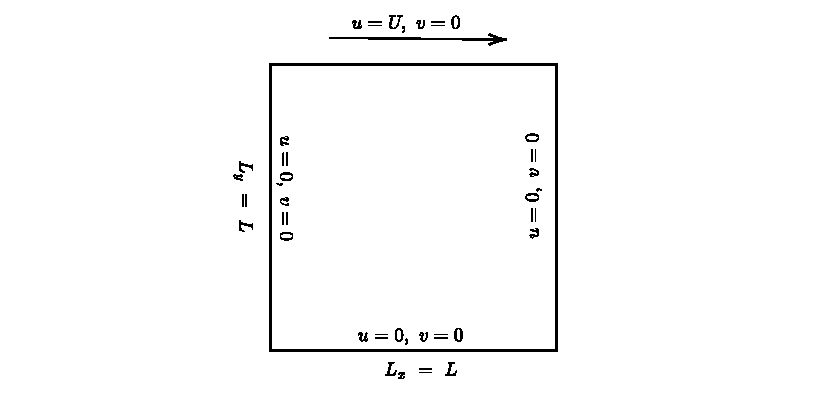
\includegraphics{lid_driven.pdf}
    \caption{Problem description of lid-driven cavity flow.}
\end{figure}

\subsection{Governing equations}
As mentioned, the flow is steady, incompressible, two-dimensional and isothermal. Therefore, 
the 2-D incompressible Navier-Stokes equations are considered, which are divided 
into the continuity equation, x-momentum equation, and y-momentum equation.

After non-dimensioning the variables as:
\begin{itemize}
    \item Length scale $x = \overline{x} L$ and $y = \overline{y} L$  
    \item  Velocity scale $u =\overline{u} U$ and $v =\overline{v} U$
    \item Pressure $p=\overline{p}\rho U^2$
\end{itemize}
The resulting governing  equations (omitting the bar notations for the sake of simplicity) are:
\begin{equation}
    \frac{\partial u}{\partial x} + \frac{\partial v}{\partial y} =0,
\end{equation}
\begin{equation}
    \label{Eq:x_mom}
    \frac{\partial u u}{\partial x} + \frac{\partial u v}{\partial y} = - \frac{dp}{dx}+\frac{1}{\text{Re}}  \left [ \frac{\partial^2 u}{\partial x^2} + \frac{\partial^2 u}{\partial y^2}\right ],
\end{equation}
\begin{equation}
    \label{Eq:y_mom}
    \frac{\partial u v}{\partial x} + \frac{\partial v v}{\partial y} = - \frac{dp}{dy}+\frac{1}{\text{Re}}  \left [ \frac{\partial^2 v}{\partial x^2} + \frac{\partial^2 v}{\partial y^2}\right ].
\end{equation}
In Eq.~\ref{Eq:x_mom} and \ref{Eq:y_mom}, Re is reynolds number of the flow, defined as:
\begin{equation}
    \text{Re}= \frac{\rho U L}{\mu},
\end{equation}
where $\mu$ is the viscosity of the fluid.

\subsection{Literature review}
Lid-driven cavity flow problem is a test case type problem for 
incompressible solvers. The past work done on lid-driven cavity 
flow gives a range for steady solution. For a wide range of 
Reynolds numbers, Shen \cite{shen1991hopf} examined the flow structures in a 
unit cavity and discovered that the flow establishes a steady 
character for Re 10000.

The difference between the projection method and the SIMPLE method 
is the projection method is generally second-order accurate, which 
is developed for the simulation of incompressible unsteady flows 
by employing a non-linear update of pressure term, which may depend 
on the grid size, time step, and even velocity. It has three and 
four-step projection method. One of the famous methods by 
Chorin~.\cite{chorin1997numerical}.The standard SIMPLE method is written 
in a concise formula for steady and unsteady flow. It is proven that SIMPLE 
type methods have second-order temporal accuracy for unsteady flows. The 
classical second-order projection method and SIMPLE type methods are 
united within the framework of the general second-order projection formula~.\cite{ni2007bridge}. 


\section{Numerical method}
This section deals with the numerical method, discretization, and grid approach in solving 
the lid-driven cavity. The SIMPLE algorithm on the staggered grid configuration 
is used. First, let’s talk about the staggered grid. 
\subsection{Staggered grid}
A staggered grid is a configuration used for spatial discretization. Scalar 
variables (such as pressure \( p \), density \( \rho \), total enthalpy \( h \), etc.) 
are stored at the cell centers of control volumes, whereas velocity components (such as 
\( u \) and \( v \)) or momentum variables are stored at the cell faces. This configuration 
differs from a collocated grid, where all variables are stored at the same locations. For 
compressible or incompressible flow simulations using structured grids, staggered storage is primarily utilized.

Collocated grids are prone to a discretization error known as odd-even 
decoupling, which leads to checkerboard oscillation patterns in the solutions. By 
using a staggered grid, odd-even decoupling between pressure and velocity can be 
effectively avoided. In a staggered grid, pressure values (\( p \)) are located at the 
center of the cells, while the velocity components \( u \) and \( v \) are stored at the cell 
faces, as shown in Fig.~\ref{}.
\begin{figure}
    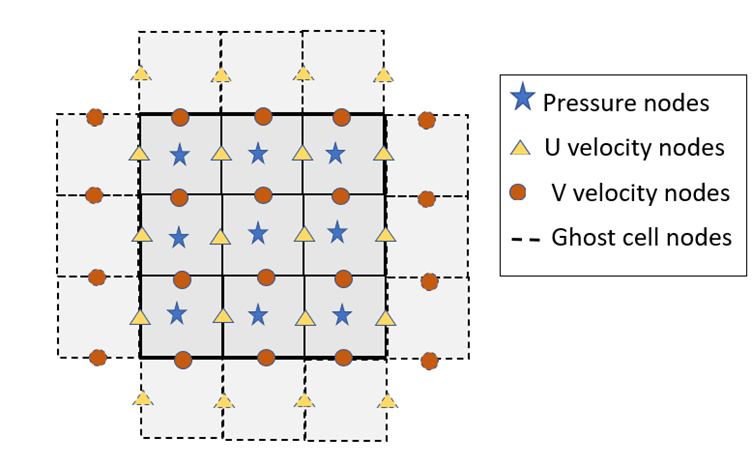
\includegraphics{\staggered_grid.png}
    \caption{Staggered grid configuration}
\end{figure}

Boundary conditions can be defined in two different forms: 
Dirichlet boundary condition, where primary variables are specified, and 
Neumann boundary condition, where derivatives, such as pressure gradients, are specified. 

To apply boundary conditions, ghost cells (cells beyond the actual computational domain) 
are introduced. Ghost cells in the \( x \)-direction are represented by dashed lines, 
which indicate the \( v \)-velocity, while those in the \( y \)-direction represent 
the \( u \)-velocity. Pressure nodes are considered in both the \( x \)- and \( y \)-
directions. The updated number of variables in the system is presented in Table~\ref{tab:variables}.

\begin{table}
    \centering
    \caption{The number of variables in the domain}
    \label{tab:variables}
    \begin{tabular}{c c c}
        \toprule
        Field quantity & Interior resolution   & Resolution with boundary points \\
        \midrule
        $p$             & $n_x \times n_y$      & $(n_x +2)\times(n_y +2)$         \\
        $u$             & $(n_x -1) \times n_y$ & $(n_x+1)\times(n_y +2) $        \\
        $v$             & $n_x \times (n_y -1)$ & $(n_x +2)\times(n_y +1)$         \\
        \bottomrule        
    \end{tabular}
\end{table}

\subsection{Discretization}
The governing equations are discretized using finite volume method. The velocity at cell center p, is approximated 
by cell centers of east e, west w, north n, and south s. The $u$  is indexing at $(i,j)$ and $v$ v at $(I,J)$. So, the $u$ momentum 
equation (Eq.~\ref{Eq:x_mom}) can be approximated as
\begin{equation}
    \frac{((u \overhat{u})_e -(u \overhat{u})_w){\Delta x}}+\frac{((u \overhat{v})_n -(u \overhat{v})_s){\Delta y}}
    = -\frac{p_{I+1,j}-p_{I-1,j}{\Delta x}}  +  \frac{1}{Re} \left [\frac{u_{i-1,j}-2u_{i,j}+u_{i+1,j}}{(\Delta x)^2} + \frac{v_{I-1,J}-2u_{I,J}+u_{I+1,J}}{(\Delta y)^2}\right ],
\end{equation}
where $u_e$,$u_w$,














\end{document}
